\begin{frame}{En resumen... nuestro prop\'osito}
    \begin{columns}
        \column{0.45\linewidth}
            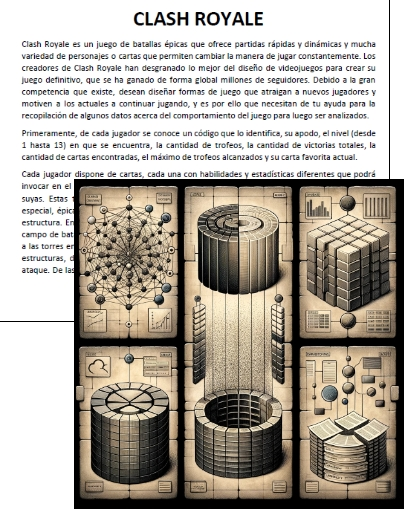
\includegraphics[width=\linewidth]{img/specs-and-dbs.jpg}
            
        \column{.1\linewidth}
            \begin{center}
                \begin{tikzpicture}
                    \node[single arrow, fill=black, inner sep=6pt] at (0,0){};
                \end{tikzpicture}
            \end{center}
            
        \column{0.45\linewidth}
            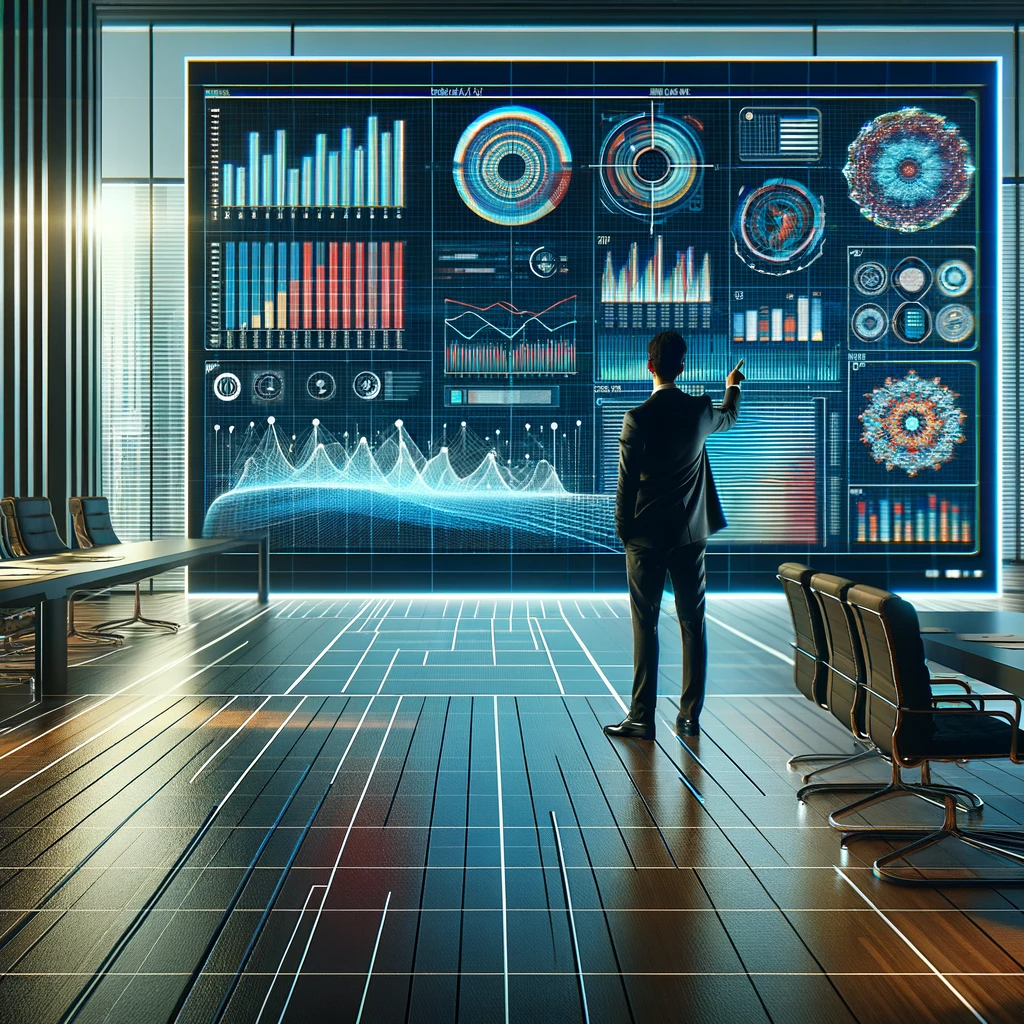
\includegraphics[width=\linewidth]{img/presenting-data.png}
        
    \end{columns}

    \note{@NOTE fin de parte. Pregunta dudas}
\end{frame}

\begin{frame}{Descripci\'on de la realidad}
    \begin{block}{¿C\'omo es una descripci\'on de la realidad?}
        \begin{enumerate}
            \item<2-> Est\'a planteada en lenguaje natural (Espa\~nol, Ingl\'es,...)
            \item<3-> Es realizada por personas con distinta formaci\'on y conocimiento
            \item<4-> Contiene una serie de \textcolor{red}{requerimientos informacionales} \begin{itemize}
                \item<5-> ¿Qu\'e datos ser\'ia de inter\'es almacenar?
                \item<6-> ¿Qu\'e restricciones o reglas se establecen sobre estos datos?
                \item<7-> ¿Qu\'e preguntas se quieren responder utilizando los datos almacenados?
            \end{itemize}
            \item<8-> Puede estar basada en cualquier \'area de la actividad humana
        \end{enumerate}
        
    \end{block}
\end{frame}